\documentclass{article}
\usepackage[utf8]{inputenc}
\usepackage{amsmath}
\usepackage{amssymb}
\usepackage{graphicx}

\begin{document}
\section*{Sequential linear systems}
We are given the following pseudocode with input $\mathbf{A}\in \mathbb{R}^{n \times n}$ and $\mathbf{b}\in \mathbb{R}^{n}$.
\begin{figure}[!hbt]
    \centering
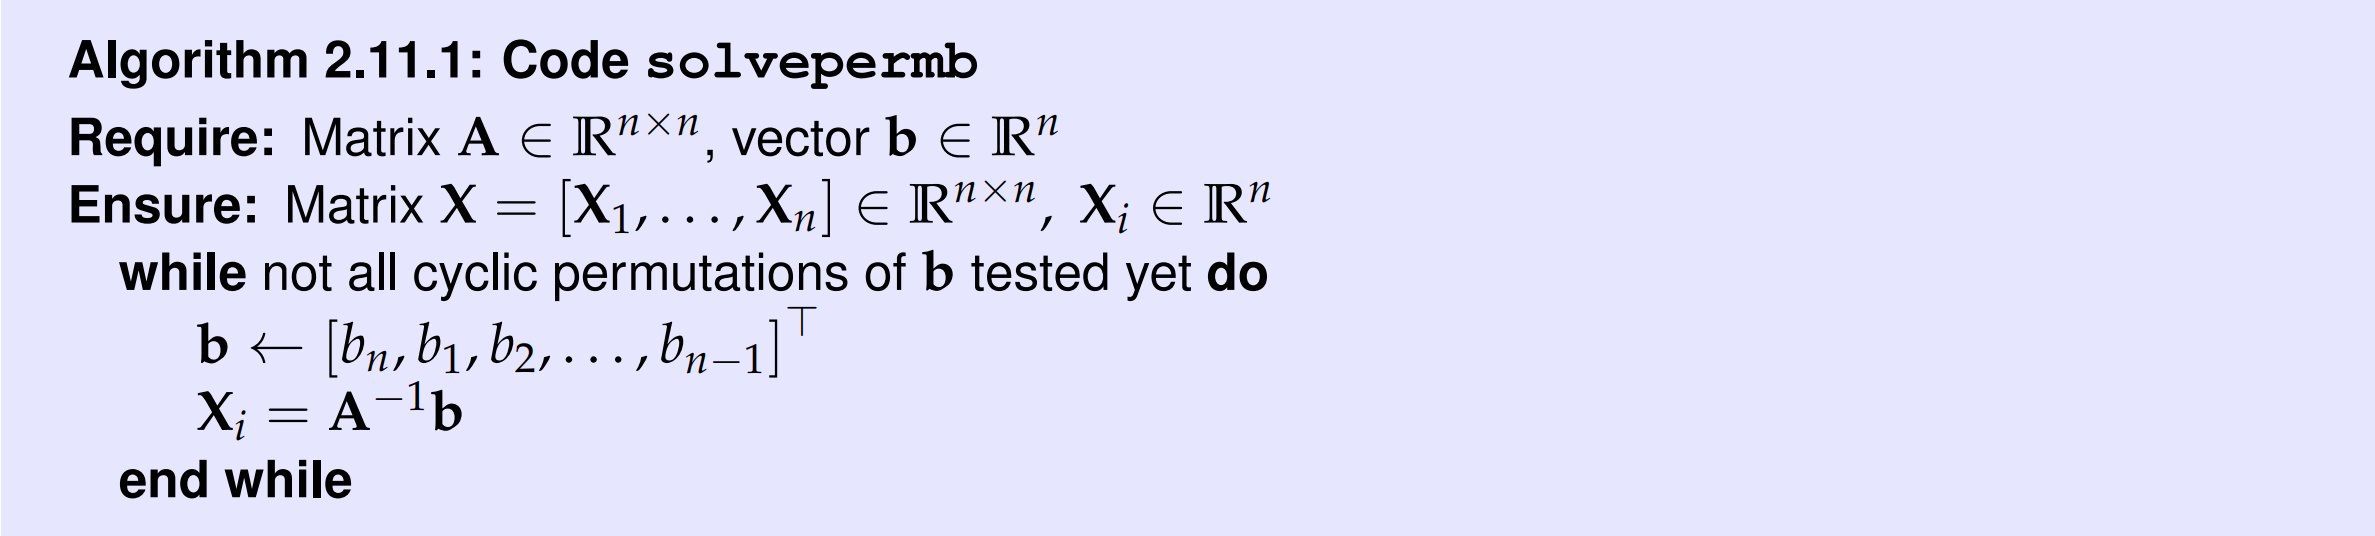
\includegraphics[width=1.0\linewidth]{2-11PseudoCode.png}
\end{figure}
\subsection*{2-11.a} 
We are tasked with giving the asymptotic complexity of the given pseudo-code. We do the computation for all cyclic permutations, there are $n$ such permutations. For each of these we solve a LSE given by $\mathbf{A}^{-1}\mathbf{b}$, which takes $\mathcal{O}\left(n^{3}\right)$ time and thus overall we get an asymptotic complexity of $\mathcal{O}\left(n^{3}\right)$.

\subsection*{2-11.b}
We are tasked with implementing the given function in Eigen. We will use a little trick to avoid actually shifting. Given the vector 
\begin{equation*}
    \left[b_{1}, b_{2}, \dots, b_{n-1}, b_{n}\right]^{\mathsf{T}}
\end{equation*}
We put a copy of the vector after the vector to give us
\begin{equation*}
    \left[b_{1}, b_{2}, \dots, b_{n-1}, b_{n}, b_{1}, b_{2}, \dots, b_{n-1}, b_{n}\right]^{\mathsf{T}}
\end{equation*}
The first few permutations are then given by
\begin{align*}
    &[b_{1}, b_{2}, \dots, b_{n-1}, b_{n},\underbrace{b_{1}, b_{2}, \dots, b_{n-1}, b_{n}}_{\text{$1$st cyclic permutation}}]^{\mathsf{T}} \\
    &[b_{1}, b_{2}, \dots, b_{n-1}, \underbrace{b_{n}, b_{1}, b_{2}, \dots, b_{n-1}}_{\text{$2$nd cyclic permutation}}, b_{n}]^{\mathsf{T}} \\
    &[b_{1}, b_{2}, \dots, b_{n-2}, \underbrace{b_{n-1}, b_{2}, \dots, b_{n-2}}_{\text{$3$rd cyclic permutation}}, b_{n-1}, b_{n}]^{\mathsf{T}} \\
\end{align*}
We can then use the Eigen utility \verb|segment(start_index, length)| to give us the necessary permutation. 

\pagebreak

This produces the following code segment.
\begin{figure}[!hbt]
    \centering
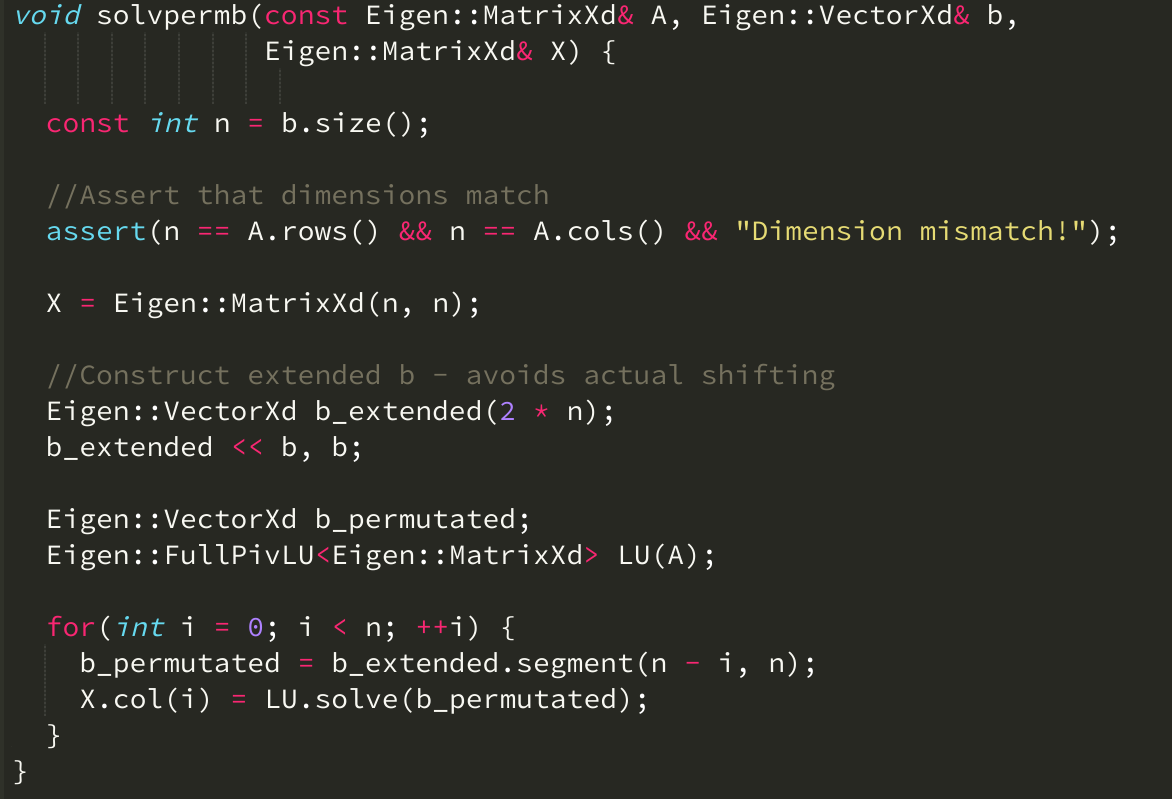
\includegraphics[width=1.0\linewidth]{2-11.b.png}
\end{figure}

\subsection*{2-11.c}
We are now tasked to implement a more efficient version of the function \verb|solvepermb| which should have asymptotic complexity $\mathcal{O}\left(n^{3}\right)$, our implementation already is in $\mathcal{O}\left(n^{3}\right)$ because we reuse the LU-decomposition, which is the only sensible thing to do. 
\end{document}
